\section{Study of Transparent Boundary Conditions in splitting methods}

\indent As an introduction for the future application of the Transparent Boundary Conditions in splitting methods, for the resolution of the wave propagation models studied in this project, we will present in this section a simple one-dimensional case, for which we will implement and qualitatively validate our proposed method. The idea is to verify if imposing independent boundary conditions for each step of the splitting method provides a good approximation for the TBCs.

\indent After this initial propose, we will work in the numerical experiment presented in \cite{halpern1986}. In this paper, approximate TBCs are implemented for a linear advection-diffusion equation with one time-dependent boundary condition, solved with a full method. Therefore, we will implement the tests described in the paper, in order to obtain the same results and compare with the solutions of the methods that we will propose.  

\subsection{Linear advection-diffusion equation}

\indent We seek to solve here the problem

\begin{equation}
	\label{eq:LinearAdvDiffEq}
	\begin{cases}
	u_t + au_x - \epsilon u_{xx} = 0, \ \ x \in \Omega = [0,1], \ \ t \ge 0  , \ \ a \in \mathbb{R}, \ \ \epsilon > 0 \\
	u(0,x) = u_0(x) = e^{-{\frac{(x-0.5)}{0.01}}^2} \\
	\text{+ boundary conditions} 		
	\end{cases} 
\end{equation}

\indent In order to focus our analysis in only one of the two boundaries, we will consider $a = 1$ (so the wave travels to the right), and choose $\epsilon = $ such that the arrival of the wave to the right boundary occurs before the arrival of the diffused solution to the left one. We will compare the results obtained with different methods :

\paragraph{Splitting method} :  The splitting method proposed here leads, in each time step $[t_n,t_{n+1}]$, to the resolution of the linear advection equation and the heat equation :

\begin{equation}
	\label{eq:operatorsSplitting}
	\begin{cases}
		L_a(v) = v_t + av_x  = 0, \ \ v^n = u^n, \ \ t \in [t_n,t_{n+1}] \\
		L_d(w) = w_t - \epsilon w_{xx} = 0, \ \ w^n = v^{n+1}, \ \ t \in [t_n,t_{n+1}]  \\
		u^{n+1} = w^{n+1}
	\end{cases}	
\end{equation}

\indent Both equations will be solved with Finite Difference methods. In the case of the linear advection, it will be an explicit backward method, with an homogeneous Dirichlet condition on the left boundary :

\begin{equation}
	\begin{cases}
		u_i^{n+1} = u_i^n - a\Delta t \frac{u_i^n - u_{i-1}^n}{\Delta x}, \ \ i = 1,...,N \\
		u_0^{n+1} = 0
	\end{cases}
\end{equation}

\indent For the heat equation, we will use the Crank-Nicolson method (semi-implicit), with homogeneous Neumann conditions in both boundaries :

\begin{equation}
\begin{cases}
\frac{u_i^{n+1}-u_i^{n}}{\Delta t} - \epsilon \frac{1}{2} \left( \frac{u_{i-1}^{n+1} - 2u_i^{n+1} + u_{i+1}^{n+1}}{\Delta x^2}  + \frac{u_{i-1}^{n} - 2u_i^{n} + u_{i+1}^{n}}{\Delta x^2} \right) = 0 \\
u_1^{n+1} = u_0^{n+1} \\
u_{N}^{n+1} = u_{N-1}^{n-1} 
\end{cases}
\end{equation}

\paragraph{Full equation} In order to compare with the results of the splitting method, we implemented a resolution of the full linear advection-diffusion equation, also with the Crank-Nicolson method, with an explicit discretization of the advection term : 

\begin{equation}
\begin{cases}
\frac{u_i^{n+1}-u_i^{n}}{\Delta t}  + a\frac{u_i^n - u_{i-1}^n}{\Delta x} - \epsilon \frac{1}{2} \left( \frac{u_{i-1}^{n+1} - 2u_i^{n+1} + u_{i+1}^{n+1}}{\Delta x^2}  + \frac{u_{i-1}^{n} - 2u_i^{n} + u_{i+1}^{n}}{\Delta x^2} \right) = 0 \\
		u_0^{n+1} = 0 \\
		B_j(u_n^{n+1}) = 0
\end{cases}
\end{equation}

\indent The boundary conditions $B_j$ are the approximate boundary conditions proposed in \cite{halpern1986}, where $j$ indicates the order of a Taylor expansion of the solutions of the characteristic equation obtained when solving  \ref{eq:LinearAdvDiffEq} in the Fourier space. We implemented here the zero and first order approximations:

\begin{equation}
	B_0 = u_x = 0 \implies u_N^{n+1} - u_{N-1}^{n+1} = 0
\end{equation}

\begin{equation}
	B_1 = u_t + u_x = 0 \implies \frac{u_N^{n+1} - u_N^{n}}{\Delta t} - \frac{u_N^{n+1} - u_{N-1}^{n+1}}{\Delta x} = 0
\end{equation}

\indent We notice that $B_0$ corresponds to an homogeneous Neumann boundary condition.

\indent We show in the figure \ref{fig:firstCase} some snapshots of the computed solutions. We compare them with a referential solution, which was computed with the full equation, using the TBC $B_1$ and in a larger domain ($\Omega_{ref} = [0,2]$). The choice of the boundary condition may not have an influence over the comparison that we intend to do here, because we will study the solution near the boundary $x=1$, which is far enough of the boundary in the referential domain.

\noindent\begin{minipage}{\textwidth} 
	\begin{minipage}{.5\textwidth} 
		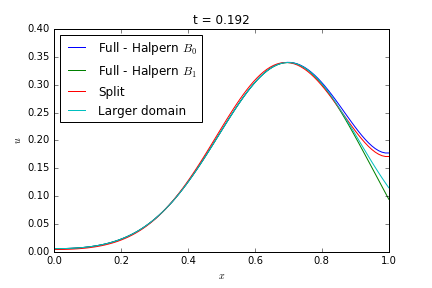
\includegraphics[scale=.48]{figures/firstCase1.png}	
		\captionof{subfigure}{Solution in the whole domain}
	\end{minipage}
	\begin{minipage}{.5\linewidth}
		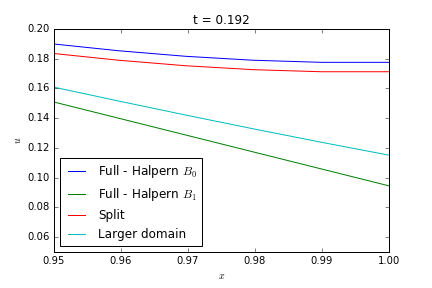
\includegraphics[scale=.48]{figures/firstCase1Detail.png}	
		\captionof{subfigure}{Detail  - right boundary}
	\end{minipage}
	\begin{minipage}{.5\textwidth} 
		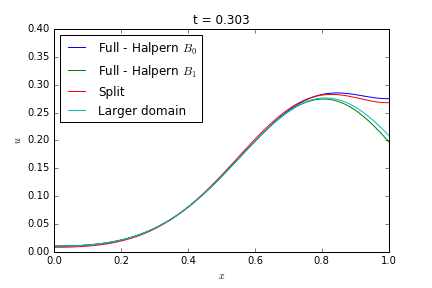
\includegraphics[scale=.48]{figures/firstCase2.png}	
		\captionof{subfigure}{Solution in the whole domain}
	\end{minipage}
	\begin{minipage}{.5\linewidth}
		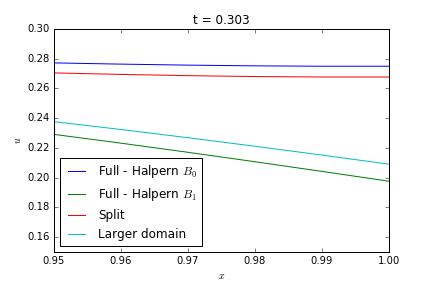
\includegraphics[scale=.48]{figures/firstCase2Detail.png}	
		\captionof{subfigure}{Detail  - right boundary}
	\end{minipage}
	\begin{minipage}{.5\textwidth} 
		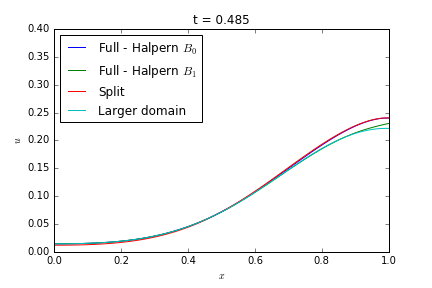
\includegraphics[scale=.48]{figures/firstCase3.png}	
		\captionof{subfigure}{Solution in the whole domain}
	\end{minipage}
	\begin{minipage}{.5\linewidth}
		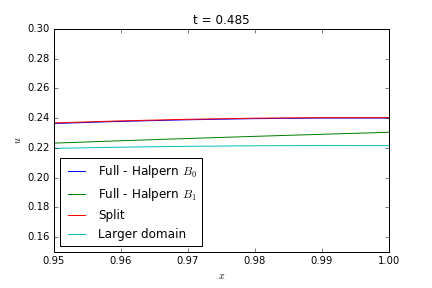
\includegraphics[scale=.48]{figures/firstCase3Detail.png}	
		\captionof{subfigure}{Detail  - right boundary}
	\end{minipage}
	\captionof{figure}{Results in different instants for the linear advection-diffusion equation, computed with a splitting method (in red) or full methods (in dark blue and green, with different approximate TBCs); also compared with a referential solution. \label{fig:firstCase}}
\end{minipage}

\indent The results of the figure \ref{fig:firstCase} shows that, compared with the referential solution, the condition $B_1$ provides a better approximation for the TBC. The full equation with $B_0$ and the splitting method provides similar but worse result, even though they qualitatively allows the solution to exit the domain without notable influence of the boundary.

\subsection{Numerical experiment realized in \cite{halpern1986}}

\indent In order to make a deeper study of the boundary conditions in splitting methods, we will implement the numerical experiment presented in \cite{halpern1986} and compare it with the solution of the splitted equation.

\indent This numerical experiment consists in the same linear advection-diffusion equation, but with zero initial conditions and a time-dependent boundary condition imposed on the left boundary :

\begin{equation}
	\label{eq:halpernProblem}
	\begin{cases}
	u_t + u_x - u_{xx} = 0, \ \ x \in \Omega = [0,1], \ \ t \ge 0  \\
	u(0,x) = 0, \ \ x \in \Omega \\
	u(t,0) = \frac{sin t}{\sqrt{t^2+1}} \\
	\text{+ right boundary conditions} 		
	\end{cases} 
\end{equation}

\indent Similarly to what we did in the previous section, \cite{halpern1986} considers a referential solution computed in the domain $
\Omega_{ref} = [0,2]$. In order to validate our implementation, we will repeat some tests presented in the paper: 

\begin{itemize}
	\item Full equation with right boundary condition $B_0$;
	\item Full equation with right boundary condition $B_1$;
	\item Transport equation (i.e, ignoring the diffusive term).
\end{itemize}

\indent We will also solve the equation using several splitting methods.  Recalling the operators defined in \eqref{eq:operatorsSplitting}, and introducing a superscript denoting the time interval in which the operator is solved, we will solve, for each time step

\begin{itemize}
	\item $L_d^{\Delta t}(L_a^{\Delta t}(u)) = 0$;
	\item $L_a^{\Delta t}(L_d^{\Delta t}(u)) = 0$;
	\item $L_a^{\Delta t/2}(L_d^{\Delta t}(L_a^{\Delta t/2}(u))) = 0$;
\end{itemize}

\noindent\begin{minipage}{\textwidth} 
	\begin{minipage}{.5\textwidth} 
		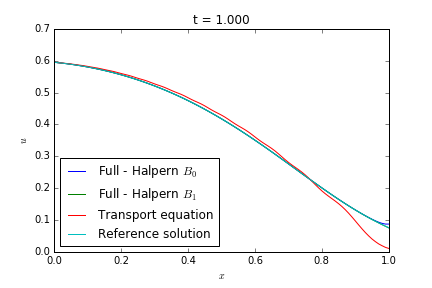
\includegraphics[scale=.48]{figures/secondCase1A.png}	
		\captionof{subfigure}{Solution in the whole domain}
	\end{minipage}
	\begin{minipage}{.5\linewidth}
		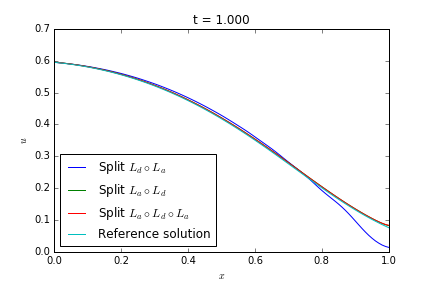
\includegraphics[scale=.48]{figures/secondCase1B.png}	
		\captionof{subfigure}{Solution in the whole domain}
	\end{minipage}
	\begin{minipage}{.5\textwidth} 
		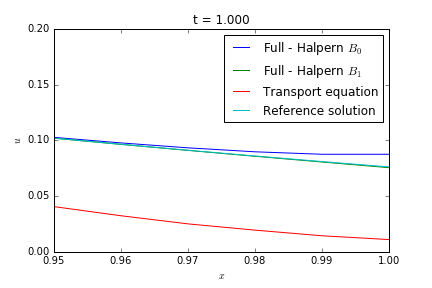
\includegraphics[scale=.48]{figures/secondCase1ADetail.png}	
		\captionof{subfigure}{Detail - right boundary}
	\end{minipage}
	\begin{minipage}{.5\linewidth}
		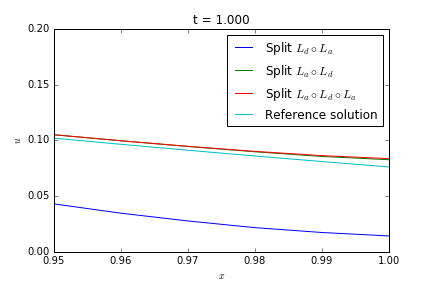
\includegraphics[scale=.48]{figures/secondCase1BDetail.png}	
		\captionof{subfigure}{Detail - right boundary}
	\end{minipage}
	\captionof{figure}{Results in $t=1$  for the numerical experiment in \cite{halpern1986}, computed with several methods and boundary conditions. \label{fig:secondCase}}
\end{minipage}

\indent Also as done in \cite{halpern1986}, we compute for each time step the error on the boundary, $e^n = u^n_N - (u_{ref})^n_N$, as shown in the figure \ref{fig:secondCaseErrors}

\noindent\begin{minipage}{\textwidth} 
	\begin{minipage}{.5\textwidth} 
		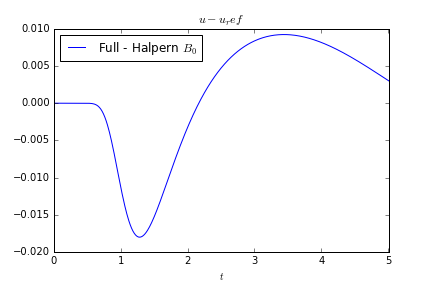
\includegraphics[scale=.48]{figures/errFullB0.png}	
		\captionof{subfigure}{Full equation with boundary condition $B_0$}
	\end{minipage}
	\begin{minipage}{.5\textwidth} 
		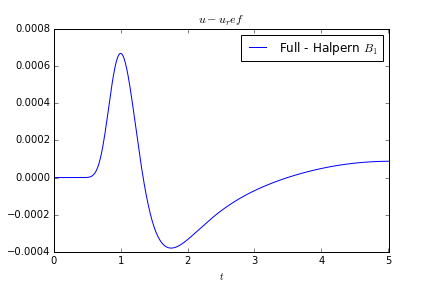
\includegraphics[scale=.48]{figures/errFullB1.png}	
		\captionof{subfigure}{Full equation with boundary condition $B_1$}
	\end{minipage}
	\begin{minipage}{.5\textwidth} 
		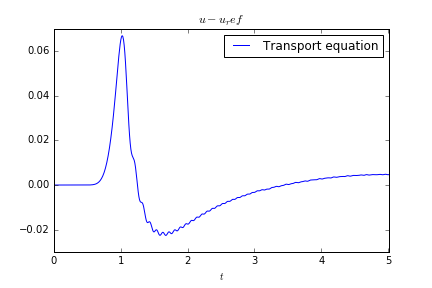
\includegraphics[scale=.48]{figures/errTransport.png}	
		\captionof{subfigure}{Transport equation}
	\end{minipage}
	\begin{minipage}{.5\textwidth} 
		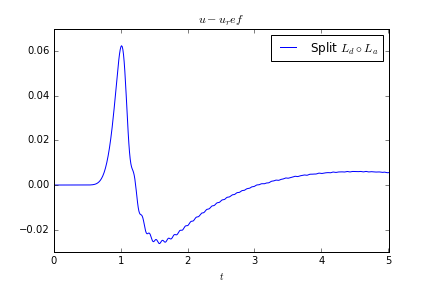
\includegraphics[scale=.48]{figures/errSplitA.png}	
		\captionof{subfigure}{Splitting  $L_d \circ L_a$}
	\end{minipage}
	\begin{minipage}{.5\textwidth} 
		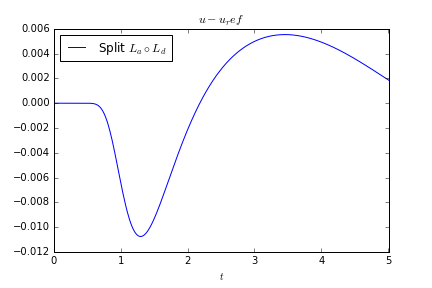
\includegraphics[scale=.48]{figures/errSplitB.png}	
		\captionof{subfigure}{Splitting  $L_a \circ L_d$}
	\end{minipage}
	\begin{minipage}{.5\textwidth} 
		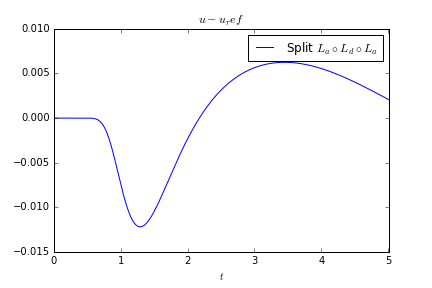
\includegraphics[scale=.48]{figures/errSplitC.png}	
		\captionof{subfigure}{Splitting  $L_a \circ L_d \circ L_a$}
	\end{minipage}
	\captionof{figure}{ Evolution of the error $e^n = u^n_N - (u_{ref})^n_N$ for each method implemented \label{fig:secondCaseErrors}}
\end{minipage}